\documentclass[11pt]{article}

% ---------- Typography and page geometry ----------
\usepackage[letterpaper,top=0.78in,bottom=0.82in,left=0.88in,right=0.88in]{geometry}
\usepackage[T1]{fontenc}
\usepackage[utf8]{inputenc}
\usepackage{amsthm}
\usepackage{newtxtext,newtxmath}
\usepackage[final]{microtype}
\usepackage{setspace}
\setstretch{1.035}
\usepackage{parskip}
\setlength{\parindent}{1.15em}
\setlength{\parskip}{0.18em}

% ---------- Mathematics ----------
\usepackage{amsmath,mathtools,bm}
\usepackage{mathrsfs}
\usepackage{bbm}
\numberwithin{equation}{section}

% ---------- Tables and figures ----------
\usepackage{booktabs,tabularx,longtable,array,multirow}
\usepackage{tikz}
\usetikzlibrary{arrows.meta,positioning,calc,fit,backgrounds}
\usepackage{caption}
\captionsetup{font=small,labelfont=bf,labelsep=period}

% ---------- Headings ----------
\usepackage{titlesec}
\titleformat{\section}{\Large\bfseries}{\thesection.}{0.55em}{}
\titleformat{\subsection}{\large\bfseries}{\thesubsection.}{0.5em}{}
\titleformat{\subsubsection}{\normalsize\bfseries}{\thesubsubsection.}{0.45em}{}
\titlespacing*{\section}{0pt}{2.15ex plus .4ex minus .2ex}{0.85ex}
\titlespacing*{\subsection}{0pt}{1.65ex plus .3ex minus .2ex}{0.55ex}

% ---------- Lists ----------
\usepackage{enumitem}
\setlist[itemize]{leftmargin=1.4em,itemsep=0.15em,topsep=0.25em}
\setlist[enumerate]{leftmargin=1.6em,itemsep=0.2em,topsep=0.25em}

% ---------- Color and links ----------
\usepackage{xcolor}
\definecolor{inkblue}{HTML}{17385F}
\definecolor{softgray}{HTML}{F4F5F7}
\definecolor{midgray}{HTML}{6D737C}
\usepackage{hyperref}
\hypersetup{
  colorlinks=true,
  linkcolor=inkblue,
  citecolor=inkblue,
  urlcolor=inkblue,
  pdfauthor={Michael Zot},
  pdftitle={Navier--Stokes: Recovering Minimal Structure from Representation-Induced Complexity},
  pdfsubject={Research repository: https://github.com/mikecreation/ZotBot/tree/main/research/navier-stokes-spc},
  pdfkeywords={Navier--Stokes, Structural Path Compression, MIPU, MAP, representation-induced complexity}
}
\usepackage[nameinlink,noabbrev]{cleveref}

% ---------- Header / footer ----------
\usepackage{fancyhdr}
\pagestyle{fancy}
\fancyhf{}
\fancyhead[L]{\small\textsc{M. Zot}}
\fancyhead[R]{\small\textsc{Structural Path Compression in Navier--Stokes}}
\fancyfoot[C]{\small\thepage}
\renewcommand{\headrulewidth}{0.35pt}
\setlength{\headheight}{14pt}

% ---------- Bibliography ----------
\usepackage[numbers,sort&compress]{natbib}
\bibliographystyle{abbrvnat}

% ---------- Theorem environments ----------
\newtheoremstyle{highend}
  {0.85em}{0.85em}{\itshape}{} {\bfseries} {.} {0.6em} {}
\theoremstyle{highend}
\newtheorem{theorem}{Theorem}[section]
\newtheorem{proposition}[theorem]{Proposition}
\newtheorem{lemma}[theorem]{Lemma}
\newtheorem{corollary}[theorem]{Corollary}
\newtheorem{principle}[theorem]{Principle}
\theoremstyle{definition}
\newtheorem{definition}[theorem]{Definition}
\newtheorem{remark}[theorem]{Remark}
\newtheorem{diagnostic}[theorem]{Diagnostic}

% ---------- Compact framed statements ----------
\usepackage{mdframed}
\newmdenv[
  linewidth=0.6pt,
  linecolor=inkblue,
  backgroundcolor=softgray,
  roundcorner=1pt,
  skipabove=0.8em,
  skipbelow=0.8em,
  innerleftmargin=10pt,
  innerrightmargin=10pt,
  innertopmargin=8pt,
  innerbottommargin=8pt
]{keybox}

% ---------- Commands ----------
\newcommand{\F}{\mathfrak F}
\newcommand{\Fadm}{\mathfrak F_{\mathrm{adm}}}
\newcommand{\X}{\mathcal X}
\newcommand{\Eret}{\mathcal E_{\mathrm{ret}}}
\newcommand{\Efull}{\mathcal E_{\mathrm{full}}}
\newcommand{\Qret}{Q_{\mathrm{ret}}}
\newcommand{\Iflat}{\mathcal I_{\mathrm{flat}}}
\newcommand{\Cl}{\operatorname{Cl}}
\newcommand{\REPROCESS}{\operatorname{REPROCESS}}
\newcommand{\dd}{\,\mathrm d}
\newcommand{\sourcepaper}{the source construction}

\begin{document}

% =====================================================================
% TITLE PAGE
% =====================================================================
\thispagestyle{empty}
\begin{center}
  \vspace*{0.38in}
  {\small\scshape Working Preprint \quad | \quad September 2026}\par
  \vspace{0.10in}
  {\fontsize{22}{26}\selectfont\bfseries
  Navier--Stokes:\\[0.12em]
  Recovering Minimal Structure from\\
  Representation-Induced Complexity\par}
  \vspace{0.22in}
  {\large Michael Zot}\par
  \vspace{0.08in}
  {\small Independent Researcher}\par
  \vspace{0.05in}
  {\small Corresponding author: \href{mailto:mike@ZotBot.Ai}{mike@ZotBot.Ai}}\par
  \vspace{0.04in}
  {\footnotesize Research repository: \href{https://github.com/mikecreation/ZotBot/tree/main/research/navier-stokes-spc}{github.com/mikecreation/ZotBot/tree/main/research/navier-stokes-spc}}\par
  \vspace{0.12in}
  \rule{0.72\textwidth}{0.45pt}\par
  \vspace{0.18in}
\end{center}

\begin{abstract}
A proof contains both mathematical dependence and the history of one successful route through a particular representation. These structures can have very different complexity. We develop \emph{Structural Path Compression}, a method for recovering a smaller generative architecture from a successful reasoning trajectory by separating same-grade dependency from higher-grade feedback. The framework is motivated by the author's earlier Minimal Irreversible Predictive Update (MIPU) and Maximal Anticipatory Pattern (MAP) formalism \cite{Zot2026MIPUMAP}.

We apply the method to the residual-improvement construction in the 2026 OpenAI Navier--Stokes blowup preprint \cite{OpenAI2026NS}. The published Section~9 construction advances a synchronized stage parameter $\sigma_j=1/5+j/10$ through a repeated correction cycle. Reorganizing the same local correction primitives about the fixed initialized state yields an admissible filtered error system. Its proposed stage-free reduction has two load-bearing estimates:
\[
K\Fadm^s\subseteq \Fadm^{s+\delta_L},
\qquad
\delta_L=\tfrac12-4\kappa_s>0,
\]
\[
\Qret(\X^s,\X^t)\subseteq \Fadm^{s+t-2\kappa_s}.
\]
For $\kappa_s=10^{-5}$, the linear return margin is $0.49996$, while the corresponding nonlinear difference gain from seed grade $\sigma_0=1/5$ is $0.19998$. Once these estimates are established, arbitrary finite residual order follows from a finite Neumann polynomial and a finite filtered Picard calculation. The existing common-domain, physical-derivative, and shrinking-cutoff arguments of the source construction can then be read through an accuracy-indexed rather than stage-indexed interface.

The mathematical claim is therefore narrower than a wholesale shortening of the 166-page source proof: the proposed compression targets the repeated residual-improvement architecture of Section~9. The broader result is methodological. A successful proof path can contain obligations created by its representation; a change of representation can delete those obligations while preserving the theorem and downstream interface. The manuscript states explicit failure criteria so that the compression can be independently audited.
\end{abstract}

\vspace{0.10in}
\noindent\textbf{Keywords.} Navier--Stokes; proof architecture; representation change; proof compression; filtered algebra; theorem proving; MIPU; MAP.\\
\textbf{MSC 2020.} 35Q30; 68T15; 68T20.\\
\textbf{Source under analysis.} OpenAI, \emph{Finite Time Blowup for Navier--Stokes}, 2026, especially Sections 7--9 \cite{OpenAI2026NS}.

\clearpage
% =====================================================================
% EXECUTIVE MATHEMATICAL MAP
% =====================================================================
\section*{Main result at a glance}
\addcontentsline{toc}{section}{Main result at a glance}

\begin{keybox}
\textbf{Structural claim.}
The repeated $+0.1$ stage schedule in Proposition~9.6 of the source construction is proposed to be replaceable, at its downstream realization interface, by a fixed-background filtered compiler once two positive return estimates are verified. The local Section~7--8 correction machinery is retained; the repeated chronological schedule is the object being removed.
\end{keybox}

\begin{figure}[h]
\centering
\resizebox{0.98\textwidth}{!}{%
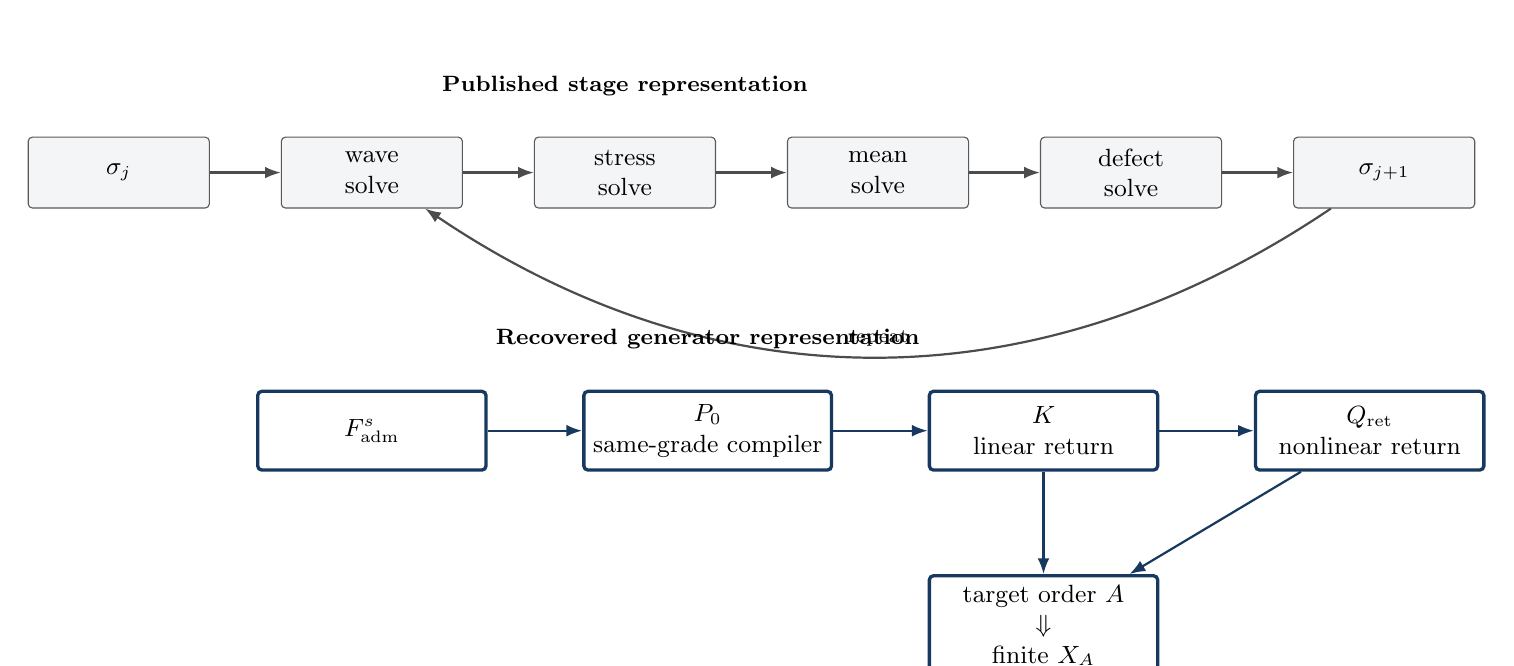
\begin{tikzpicture}[
  node distance=8mm and 9mm,
  every node/.style={font=\small,align=center},
  box/.style={draw=black!65,rounded corners=1.5pt,minimum height=9mm,minimum width=23mm,fill=softgray},
  main/.style={draw=inkblue,very thick,rounded corners=1.5pt,minimum height=10mm,minimum width=29mm,fill=white},
  arr/.style={-{Latex[length=2mm]},thick,draw=black!70}
]
\node[box] (sj) {$\sigma_j$};
\node[box,right=of sj] (wave) {wave\\solve};
\node[box,right=of wave] (stress) {stress\\solve};
\node[box,right=of stress] (mean) {mean\\solve};
\node[box,right=of mean] (def) {defect\\solve};
\node[box,right=of def] (sj1) {$\sigma_{j+1}$};
\draw[arr] (sj)--(wave); \draw[arr] (wave)--(stress); \draw[arr] (stress)--(mean); \draw[arr] (mean)--(def); \draw[arr] (def)--(sj1);
\draw[arr,bend left=34] (sj1) to node[above,font=\scriptsize] {repeat} (wave);
\node[font=\footnotesize\bfseries,above=4mm of stress] {Published stage representation};

\node[main,below=23mm of wave] (filt) {$\Fadm^s$};
\node[main,right=12mm of filt] (p0) {$P_0$\\same-grade compiler};
\node[main,right=12mm of p0] (ret) {$K$\\linear return};
\node[main,right=12mm of ret] (qa) {$\Qret$\\nonlinear return};
\draw[arr,draw=inkblue] (filt)--(p0); \draw[arr,draw=inkblue] (p0)--(ret); \draw[arr,draw=inkblue] (ret)--(qa);
\node[main,below=13mm of ret] (A) {target order $A$\\$\Downarrow$\\finite $X_A$};
\draw[arr,draw=inkblue] (ret)--(A); \draw[arr,draw=inkblue] (qa)--(A);
\node[font=\footnotesize\bfseries,above=4mm of p0] {Recovered generator representation};
\end{tikzpicture}%
}
\caption{The proposed representation change. The source construction synchronizes several unequal gains through a repeated $+0.1$ stage clock. The compressed representation attempts to expose the same-grade finite dependency graph and treat all returns by their positive filtration degree.}
\label{fig:architecture}
\end{figure}

\begin{proposition}[Two load-bearing estimates]\label{prop:two-estimates}
Let $U_0$ denote the initialized state of Proposition~9.5 of the source construction. If the legal one-pass compiler $P_0$ and the retained fixed-background error expansion satisfy
\[
K:=I+L_{\mathrm{ret}}P_0,
\qquad
K\Fadm^s\subseteq \Fadm^{s+\frac12-4\kappa_s},
\]
and
\[
\Qret(\X^s,\X^t)\subseteq \Fadm^{s+t-2\kappa_s},
\]
then every finite target grade $A>1/5$ admits a finite legal correction $X_A$ whose retained error lies in $\Fadm^A$, modulo flat pulse/cutoff remainders. The remaining passage to a smooth field uses the same common-domain, derivative-loss, and shrinking-cutoff interfaces already present in the source construction.
\end{proposition}

\noindent The paper is deliberately organized so that an independent reader can attack \cref{prop:two-estimates} without accepting the conceptual narrative surrounding it.

\tableofcontents
\clearpage

% =====================================================================
\section{The complexity of a theorem and the complexity of reaching it}
A proof has at least two geometries: the geometry of mathematical dependence and the geometry of the route by which that dependence was discovered. A long successful trajectory establishes reachability; it does not by itself establish that every part of the trajectory belongs to the irreducible structure of the problem.

This distinction becomes sharper when mathematical discovery is computational. A machine can search a vast space of intermediate states, repeatedly repairing obligations created by one representation, before a later analysis recognizes that those obligations are generated by a much smaller rule. The resulting post-discovery question is
\[
\boxed{\text{Which parts of a successful proof belong to the problem, and which belong to the representation?}}
\]

The present paper studies that question in the residual-improvement machinery of the OpenAI Navier--Stokes construction \cite{OpenAI2026NS}. The source paper is 166 pages; its Section~9 occupies printed pages 100--115 and coordinates local operators already developed in Sections~7--8. On printed page 106 the authors state that the base, primary amplitudes, and inverse operators are kept fixed throughout the correction construction; Proposition~9.6 then repeats the four-step cycle and advances all tracked orders by $0.1$ \cite[pp.~106--111]{OpenAI2026NS}. Lemmas~9.7--9.8 provide the common physical domain and derivative-loss interface used by Proposition~9.9 \cite[pp.~111--115]{OpenAI2026NS}.

The aim here is not to rewrite the complete Navier--Stokes proof. It is to identify whether the Section~9 stage schedule is an intrinsic mathematical grade or a synchronization grade introduced by the chosen proof organization.

\subsection{Persistent information and inferential closure}
Let $D$ denote a mathematical state and $R$ a representation. We write
\[
\Cl_R(D)
\]
for the consequences accessible from $D$ under the transformations made natural by $R$. Two representations can preserve the relevant mathematical content while exposing different amounts of immediate consequence:
\[
R_1(D)\simeq R_2(D),
\qquad
\Cl_{R_1}(D)\subsetneq \Cl_{R_2}(D).
\]
Nothing new has been measured. The inferential closure has changed. Change-of-representation research in automated reasoning explicitly studies this phenomenon \cite{Raggi2016,HolteZimmerMacDonald1992}; proof planning similarly separates reusable high-level proof structure from low-level inference search \cite{Bundy1988}.

\begin{definition}[Representation-induced complexity]
Representation-induced complexity is proof or search work that disappears under a faithful recoding while the hypotheses, conclusion, and downstream mathematical interface remain intact.
\end{definition}

\begin{remark}
This definition is intentionally operational. It does not require a universal numerical measure of complexity. Deletion of an independent proof obligation is already evidence that some work belonged to the representation rather than the theorem's invariant dependency structure.
\end{remark}

% =====================================================================
\section{MIPU, MAP, and Structural Path Compression}
The conceptual language used here develops the author's earlier MIPU/MAP framework \cite{Zot2026MIPUMAP}. A \emph{Minimal Irreversible Predictive Update} (MIPU) is a smallest integrated update that changes what can be predicted or inferred next. A \emph{Maximal Anticipatory Pattern} (MAP) is the widest coherent predictive structure supported by the information currently available.

For proofs, the translation is natural. A proof MIPU changes the future deductive state. A proof MAP is a stable dependency architecture that predicts an entire family of later steps.

\begin{keybox}
\textbf{Core law.}
\[
\text{successful trajectory}\neq\text{minimum sufficient trajectory}.
\]
A sequence of valid local updates can eventually reveal a generator that makes future instances of those updates predictable rather than independently proved.
\end{keybox}

\subsection{Reprocess under recode}
If a new representation $R_2$ enlarges the inferential closure of already possessed information $D$, then conclusions extracted under $R_1$ should not simply be carried forward unchanged. The original material should be revisited:
\[
R_1\to R_2
\quad\Longrightarrow\quad
\REPROCESS(D).
\]
A previously necessary-looking proof step may become a derived consequence. A repeated cycle may become a finite expansion of one transfer law. This operation is the bridge from MIPU/MAP to Structural Path Compression.

\subsection{Horizontal and vertical structure}
The central diagnostic is to separate \emph{same-grade} dependence from \emph{higher-grade} feedback. If the current-grade graph is acyclic, all obligations at that grade can be solved by finite forward substitution. If every return edge has strictly positive degree, repetition survives only as a move to higher filtration.

The target pattern is therefore
\[
\boxed{\text{acyclic horizontally, increasing vertically}.}
\]
This pattern is what the Navier--Stokes case appears to exhibit.

% =====================================================================
\section{The source architecture under analysis}
Section~9 of \cite{OpenAI2026NS} assembles four correction mechanisms developed earlier in the paper:
\begin{enumerate}
  \item a supported nonzero-harmonic pulse inverse (Proposition~7.2, printed p.~77);
  \item a signed covariance/stress realization (Proposition~7.6, printed p.~84);
  \item compactly supported mean corrections and exact compatibility identities (Section~8, especially Proposition~8.4 and Corollary~8.5, printed pp.~94--95);
  \item a fixed five-equation compatibility correction (Lemmas~8.7--8.8, printed pp.~97--99).
\end{enumerate}

Proposition~9.1 and Lemma~9.2 then quantify the residual and product orders created by these operations \cite[pp.~101--103]{OpenAI2026NS}. Proposition~9.3 explicitly permits any \emph{finite sequence} of the named primitive corrections around the fixed slow base and primary waves, provided pressure is reconstructed from the complete current velocity and nonlinear products use the complete current field \cite[pp.~103--105]{OpenAI2026NS}.

\subsection{The published stage clock}
Definition~9.4 uses
\[
B_j=\frac12+\sigma_j,
\qquad
C_j^*=1+\sigma_j,
\qquad
\sigma_j=\frac15+\frac{j}{10}.
\]
Proposition~9.6 performs the wave, averaged-stress, zero-average mean, and compatibility corrections, then shows that all tracked orders improve by $0.1$. The closing page of the proposition explicitly takes the minimum of several larger gains and concludes that the wave, tangential mean, and defect orders all improve by $0.1$ \cite[p.~111]{OpenAI2026NS}.

This is the first structural clue: the $0.1$ increment is a common synchronization rate, not the exact gain of the individual return channels.

% =====================================================================
\section{Admissible filtration and recovered dependency graph}
Freeze the initialized state $U_0=(u^{[0]},p^{[0]})$. The retained augmented error is organized into
\[
W,\qquad \bar M,\qquad M^\circ,\qquad S,
\]
where $W$ is the nonzero angular-harmonic residual, $\bar M$ is the auxiliary-averaged tangential mean residual, $M^\circ$ is its zero-auxiliary-average complement, and $S$ stores the compact-support compatibility state $(P,J_\theta,J_z)$.

Define
\begin{equation}\label{eq:filtration}
\F^s=
W_{\frac12+s}
\oplus
\bar M_{1+s-\kappa_s}
\oplus
M^\circ_{1+s-2\kappa_s}
\oplus
S_{1+s-2\kappa_s}.
\end{equation}
The actual compiler domain is the admissible subspace $\Fadm^s$ satisfying the exact integrated identities inherited from Proposition~8.4:
\[
\int R^2\bar E_\theta\,\dd R=\varepsilon\partial_ZJ_\theta,
\qquad
\int R\bar E_z\,\dd R=\varepsilon\partial_Z(J_z+c_\rho P).
\]
These relations are needed to prepare the compact stress target used by the signed-wave inverse.

\subsection{The same-grade graph}
At fixed grade the principal ordering is
\[
\boxed{W\longrightarrow \bar M\longrightarrow M^\circ\longrightarrow S.}
\]
There are shortcut arrows, but every same-grade dependency moves forward. The reverse arrows are higher-order returns.

The one-pass compiler $P_0$ is the finite forward substitution through this graph, using exactly the primitive operations admitted by Proposition~9.3: pulse inverse and curl, signed-stress correction, zero-average mean inverse, compatibility correction, with pressure reconstructed from the complete updated velocity after each update. No new inverse family is introduced.

The loss parameter is not chosen by the present manuscript. The source fixes
\[
\kappa_s=10^{-5}
\]
in equation~(6.2) and repeats this convention at the beginning of Section~9 \cite[pp.~63,100]{OpenAI2026NS}.

Let
\[
K:=I+L_{\mathrm{ret}}P_0.
\]
The central linear statement is
\begin{equation}\label{eq:linear}
K\Fadm^s\subseteq \Fadm^{s+\delta_L},
\qquad
\delta_L=\frac12-4\kappa_s.
\end{equation}

\begin{lemma}[Source-addressed linear return]\label{lem:linear-trace}
For the filtration \eqref{eq:filtration}, every linear return produced by one legal pass has strictly positive relative degree. The smallest degree is
\[
\delta_L=\frac12-4\kappa_s=0.49996.
\]
\end{lemma}

\begin{proof}
Write $B=\frac12+s$. For a supported wave source in $W_B$, Proposition~9.1 leaves supported linear residual in
\[
W_{B+\frac12-3\kappa_s},
\]
so the $W\to W$ return gains $\frac12-3\kappa_s$ \cite[pp.~101--102]{OpenAI2026NS}.

For the averaged-mean sector, admissibility and Corollary~8.5 prepare the auxiliary-independent compact stress target. Proposition~7.6 maps a stress in $M^\alpha$ to the typed signed-wave image $W^{\alpha-1/2}$ and gives the exact covariance identity $B(W_0,L\Sigma)=\Sigma$ \cite[pp.~84--85]{OpenAI2026NS}. With input threshold
\[
\bar M_{1+s-\kappa_s},
\]
the resulting signed correction has the conservative wave exponent $B-\kappa_s$. Proposition~9.1 then gives its linear residual at
\[
W_{B+\frac12-4\kappa_s}
=
W_{1+s-4\kappa_s}.
\]
This is exactly the $W$ component of $\F^{s+\frac12-4\kappa_s}$. The same exponent appears explicitly in Step~2 of Proposition~9.6, where the signed correction lies in $W_{B-\kappa_s}$ and its linear error has exponent $B+\frac12-4\kappa_s$ \cite[pp.~109--110]{OpenAI2026NS}. This is the bottleneck return.

For $M^\circ$, put $H=1+s-2\kappa_s$. Lemma~8.6 and Step~3 of Proposition~9.6 produce the zero-average mean correction in $M_H$; its interaction with the fixed wave field returns a wave in $W_H$, while the remaining mean residual gains to $M_{H+1-2\kappa_s}$ \cite[pp.~96,110]{OpenAI2026NS}. The wave return therefore has relative degree $\frac12-2\kappa_s>\delta_L$.

For the compatibility sector $S_H$, Lemmas~8.7--8.8 and Step~4 of Proposition~9.6 cancel the linear defect and leave the compatibility remainder in
\[
S_{H+0.9-2\kappa_s},
\]
which has relative degree $0.9-2\kappa_s>\delta_L$ \cite[pp.~97--99,111]{OpenAI2026NS}. Pressure reconstruction is the fixed exact map of Section~8 and the source recomputes it after every update. Thus no linear return has degree below $\delta_L$.
\end{proof}

% =====================================================================
\section{Source-addressed quadratic return}
The second load-bearing estimate concerns the physical quadratic map. The compiler keeps typed provenance internally. In particular, the exact identity $B(W_0,L\Sigma)=\Sigma$ belongs only to the signed-stress image of Proposition~7.6, not to an arbitrary wave that happens to satisfy the same norm bound.

For a correction generated from grade $s$, use the conservative source envelopes
\[
\X^s:\qquad
w\in W_{\frac12+s-\kappa_s},
\qquad
m_{\mathrm{tan}}\in M_{1+s-2\kappa_s},
\]
with the radial mean one order better, as in the source mean classes. These envelopes contain the actual one-pass corrections; the $-\kappa_s$ in the wave exponent accounts for the signed-stress branch, which is the lowest wave correction produced by the pass.

\begin{lemma}[Source-addressed quadratic return]\label{lem:quadratic-trace}
For realized corrections in the preceding typed envelopes,
\begin{equation}\label{eq:quadratic}
\Qret(\X^s,\X^t)\subseteq \Fadm^{s+t-2\kappa_s}.
\end{equation}
The equality case in the filtration bookkeeping is the same-label wave--wave zero harmonic.
\end{lemma}

\begin{proof}
Let
\[
\alpha=\frac12+s-\kappa_s,
\qquad
\alpha'=\frac12+t-\kappa_s.
\]
Lemma~9.2 gives the zero angular harmonic of two same-label curl-generated waves in
\[
M_{\alpha+\alpha'-\kappa_s}
=
M_{1+s+t-3\kappa_s}.
\]
The $\bar M$ component of the target filtration is
\[
\bar M_{1+(s+t-2\kappa_s)-\kappa_s}
=
\bar M_{1+s+t-3\kappa_s},
\]
so this channel exactly saturates \eqref{eq:quadratic}. The nonzero wave--wave harmonic has the same source exponent $1+s+t-3\kappa_s$, which lies strictly above the required wave threshold
\[
W_{\frac12+s+t-2\kappa_s}.
\]
These statements are precisely the two wave--wave conclusions of Lemma~9.2 \cite[pp.~102--103]{OpenAI2026NS}.

For a wave of exponent $\alpha$ and a tangential mean of exponent
\[
\mu=1+t-2\kappa_s,
\]
Lemma~9.2 gives the nonzero harmonic in
\[
W_{\alpha+\mu-1/2}
=
W_{1+s+t-3\kappa_s},
\]
again strictly above the required wave threshold by $\frac12-\kappa_s$. Distinct labels have zero products on their closed supports by the final statement of Lemma~9.2. The remaining mean--mean and compatibility products are higher order in the exact Section~8 equations; the same ordering is recorded explicitly in Steps~3--4 of Proposition~9.6, where the uncancelled mean and defect products gain at least the displayed positive margins \cite[pp.~110--111]{OpenAI2026NS}. Proposition~9.3 preserves the exact compatibility identities and retained/flat decomposition after every finite legal sequence, so the output remains in the admissible subspace.
\end{proof}

Since the initialized source state has $\sigma_0=1/5$, the nonlinear difference gain is
\[
\eta=\sigma_0-2\kappa_s=0.19998>0.
\]
The resulting architecture is summarized by two positive return margins:
\[
\boxed{\delta_L=0.49996,\qquad \eta=0.19998.}
\]

\begin{table}[h]
\centering
\caption{Critical channels and their source addresses.}
\label{tab:criticalchannels}
\begin{tabularx}{\textwidth}{@{}p{0.12\textwidth}p{0.29\textwidth}Xp{0.16\textwidth}@{}}
\toprule
Type & Channel & Source inheritance & Margin \\
\midrule
Linear & $\bar M\to$ signed-stress wave $\to W$ & Proposition~7.6 + Proposition~9.1; Proposition~9.6 Step~2 displays $B+1/2-4\kappa_s$ & $\frac12-4\kappa_s$ \\
Quadratic & $W\times W\to\bar M$ & Lemma~9.2 gives $M_{\alpha+\alpha'-\kappa_s}$ & seed gain $\frac15-2\kappa_s$ \\
Linear & $M^\circ\to W$ & Lemma~8.6 + Proposition~9.6 Step~3 & $\frac12-2\kappa_s$ \\
Linear & $S\to S$ after defect solve & Lemmas~8.7--8.8 + Proposition~9.6 Step~4 & $0.9-2\kappa_s$ \\
\bottomrule
\end{tabularx}
\end{table}

% =====================================================================
\section{Finite algebra replaces infinite staging}
Fix a target grade $A>\sigma_0$ and set
\[
N_A:=\min\{N:\sigma_0+N\delta_L\ge A\}.
\]
Define the finite polynomial
\begin{equation}\label{eq:PA}
P_A=P_0\sum_{n=0}^{N_A-1}K^n.
\end{equation}
Because $L_{\mathrm{ret}}P_0=K-I$,
\[
L_{\mathrm{ret}}P_A=K^{N_A}-I.
\]
Thus $P_A$ is an inverse to the required finite resolution; no infinite Neumann series or new completion is required.

\subsection{A literal source-legal compiler expansion}
The abstract polynomial can be expanded into the primitive operations permitted by Proposition~9.3. For a concrete target, take $A=1$. Since
\[
\sigma_0+\delta_L=0.69996<1,
\qquad
\sigma_0+2\delta_L=1.19992>1,
\]
we have $N_1=2$ and therefore
\[
P_1e=P_0e+P_0Ke.
\]
The first term $P_0e$ is executed as the following finite block:
\begin{enumerate}
  \item apply Proposition~7.2 and the curl construction to the current supported $W$ source;
  \item reconstruct pressure from the complete updated velocity by the Section~8 pressure map;
  \item use Corollary~8.5 to prepare the compact averaged stress and Proposition~7.6 for the typed signed-stress correction;
  \item reconstruct pressure;
  \item apply Lemma~8.6 to the zero-auxiliary-average mean source;
  \item reconstruct pressure;
  \item apply the fixed compatibility correction of Lemmas~8.7--8.8;
  \item reconstruct pressure and form the retained plus flat decomposition of Proposition~9.3.
\end{enumerate}
The retained linear error after this block is $Ke$. The second term $P_0Ke$ is obtained by applying the same eight-step block to that higher-grade retained source. Proposition~9.3 explicitly permits arbitrary finite sequences of these named primitives around the fixed slow base and primary waves, provided pressure is recomputed and products use the complete current fields \cite[pp.~103--105]{OpenAI2026NS}. Hence $P_1$ introduces no new inverse and no operation outside the source-legal primitive family. The same argument expands every finite $P_A$, and every call to $P_A$ inside the finite nonlinear iteration expands into the same finite primitive block.

The nonlinear correction is computed by finite filtered Picard substitution:
\[
Y_A^{(m+1)}=e_0+\Qret(P_AY_A^{(m)},P_AY_A^{(m)}).
\]
Successive differences gain at least $\eta>0$, so after finitely many substitutions the iteration stabilizes modulo $\F^A$. Setting $X_A=P_AY_A$ yields
\[
\Efull(U_0+X_A)\in \Fadm^A+\Iflat.
\]

The key conceptual shift is therefore
\[
\boxed{\text{stage number }j\quad\longrightarrow\quad\text{requested accuracy }A.}
\]
Accuracy becomes an input to a finite generator rather than an inherited consequence of repeatedly advancing a clock.

% =====================================================================
\section{Returning to physical space}
The source proof's Lemmas~9.7--9.8 are the last place where the deleted stage parameter could be carrying hidden analytic work. Lemma~9.7 gives one $q_{\mathrm{big}}>0$ independent of stage and derivative order; its proof attributes this uniformity to the fixed background, fixed primary covariance, fixed supports, and fixed inverse operators \cite[pp.~111--113]{OpenAI2026NS}. Lemma~9.8 gives physical derivative bounds with exponent losses independent of stage and only afterward inserts the specific stage fact that every retained increment has normalized exponent at least $j/10$ \cite[pp.~113--114]{OpenAI2026NS}.

The stage-free reading replaces that specific normalized exponent by the shell order $A_{j-1}$ of an increasing accuracy sequence $A_j\to\infty$. Consequently one obtains correction orders and residual orders tending to infinity with fixed derivative losses, which is precisely the interface required by Lemma~5.4 and Proposition~9.9 \cite[pp.~56--61,114--115]{OpenAI2026NS}.

\begin{theorem}[Stage-free replacement at the downstream interface]\label{thm:replacement}
Assume \eqref{eq:linear} and \eqref{eq:quadratic}, together with legality of $P_0$, preservation of admissibility, and the stage-free extraction of the common-domain and physical-derivative estimates from Lemmas~9.7--9.8 of \cite{OpenAI2026NS}. Then the repeated law
\[
\sigma_{j+1}=\sigma_j+\frac1{10}
\]
is unnecessary for producing the hypotheses consumed by the final shrinking-cutoff realization. Any sequence $A_j\to\infty$ generates finite legal states whose shell orders and physical residual orders tend to infinity with derivative losses independent of $j$.
\end{theorem}

% =====================================================================
\section{What has actually been compressed}
The local PDE machinery remains. The oscillatory inverse remains. The signed covariance realization remains. The mean inverse remains. The compatibility correction remains. Pressure reconstruction remains. Product estimates, support calculus, and the final shrinking-cutoff theorem remain.

What disappears is the need to use the particular repeated schedule
\[
\sigma_j=\frac15+\frac{j}{10}
\]
as the primitive explanation of residual improvement.

\begin{table}[h]
\centering
\caption{Scope ledger: what is retained, replaced, and removed.}
\label{tab:scopeledger}
\begin{tabularx}{\textwidth}{@{}p{0.34\textwidth}p{0.17\textwidth}X@{}}
\toprule
Source architecture & SPC treatment & Reason \\
\midrule
Sections~7--8 local pulse, stress, mean, compatibility, and pressure machinery & retained & These are the primitive operators compiled by $P_0$. \\
Proposition~9.3 finite-sequence legality & retained & It is the execution/type interface for finite compiler outputs. \\
Proposition~9.6 chronological $+0.1$ stage clock & replaced & Return channels are indexed by their actual filtration gains rather than a common synchronization increment. \\
Stage genealogy $j\mapsto j+1$ as the driver of accuracy & replaced & Target accuracy $A$ determines the finite polynomial depth $N_A$. \\
Lemmas~9.7--9.8 common-domain and derivative-loss interface & retained & They provide the stage-independent analytic interface consumed by final realization. \\
Proposition~9.9 and Lemma~5.4 realization & retained & The downstream theorem interface is unchanged. \\
Flat pulse/cutoff remainder & retained separately & It remains outside the finite-order compiler state. \\
\bottomrule
\end{tabularx}
\end{table}

\begin{keybox}
\textbf{Structural compression is measured by deleted obligations, not deleted pages.}
The proposed reduction does not turn a 166-page proof into three pages. It targets a specific repeated proof architecture inside Section~9. Its significance, if verified, is that infinitely many synchronized stage obligations become consequences of two reusable filtration estimates.
\end{keybox}

This distinction also clarifies why the source construction can be locally efficient and globally compressible at the same time. Proposition~9.6 already compresses several unequal gains into one safe $+0.1$ clock. Structural Path Compression asks whether that clock itself must be replayed once the return law has been isolated.

% =====================================================================
\section{Representation-induced complexity and mathematical understanding}
Classical proof complexity studies shortest proof length relative to formal systems \cite{CookReckhow1979}. Proof planning studies reusable high-level patterns that organize lower-level inference \cite{Bundy1988}. Automated change-of-representation work studies how equivalent encodings alter reasoning performance \cite{Raggi2016,HolteZimmerMacDonald1992}. Thurston's discussion of mathematical progress emphasizes that understanding is not exhausted by possession of a formal derivation \cite{Thurston1994}.

Structural Path Compression treats a successful proof as data for a second discovery problem:
\[
\boxed{\text{What compact structure explains why this trajectory kept succeeding?}}
\]
A long machine-generated proof can therefore be both a certificate and a measurement of the problem under one representation.

\subsection{Discovery, structure, representation, verification}
It is useful to distinguish four costs:
\[
C_{\mathrm{discovery}},\qquad C_{\mathrm{structure}},\qquad C_{\mathrm{representation}},\qquad C_{\mathrm{verification}}.
\]
Observed reasoning length is not a direct measurement of intrinsic structure. Expensive search can discover a small generator. Conversely, a concise presentation can hide substantial search or representation cost.

\subsection{Machine-generated mathematics}
Recent formal theorem-proving systems such as AlphaProof demonstrate the power of learned search in formally verified environments \cite{AlphaProof2025}. The natural post-solution extension is
\[
\text{search}\to\text{verify}\to\text{extract dependencies}\to\text{search representations}\to\text{compress}\to\text{reprocess}.
\]
The relevant long-run question becomes less ``can the system reason far enough?'' and more ``can it discover why so much of its own reasoning was unnecessary?''

% =====================================================================
\section{Falsification surface}
A compression of a major proof should become easier to attack after reformulation, not harder. The present proposal fails if any of the following is established:
\begin{enumerate}
  \item a zero-degree cycle exists in the same-grade dependency graph;
  \item $P_0$ applies any primitive inverse outside its domain;
  \item the signed covariance identity is used for an untyped generic wave rather than a wave in the image of Proposition~7.6;
  \item $\Qret$ fails to preserve the admissibility identities;
  \item an overlooked nonlinear channel removes the positive margin $\eta$;
  \item exact pressure reconstruction introduces algebraic degree greater than two around $U_0$;
  \item a finite compiler output cannot be expanded into a legal finite sequence of the operations permitted by Proposition~9.3;
  \item flat remainders can re-enter finite order under one of the allowed finite operations;
  \item the common physical domain shrinks with target accuracy;
  \item physical exponent losses grow with target order;
  \item the downstream summation uses genealogical information specific to the original stage sequence;
  \item higher target accuracy modifies lower-order shells, so $X_B-X_A\notin\X^A$ for some $B>A$.
\end{enumerate}

\begin{diagnostic}[Fastest route to disproof]
The mathematically cheapest way to kill the proposed compression is to exhibit one legal same-grade feedback loop of total degree zero. The second-cheapest is to exhibit one quadratic channel whose loss is large enough to make $\eta\le0$.
\end{diagnostic}

% =====================================================================
\section{Audit and reproducibility protocol}
The manuscript is designed for independent checking at three levels.

\subsection{Source fidelity audit}
Every primitive operator invoked by the compiler is tied to its exact source proposition or lemma in \cite{OpenAI2026NS}. Appendix~\ref{app:crosswalk} records the source statement, the typed role, and the exponent inherited by the compiler. In particular, \cref{lem:linear-trace,lem:quadratic-trace} give the two master-inclusion traces in the body of the paper.

\subsection{Channel audit}
Every arrow entering or leaving $W,\bar M,M^\circ,S$ is assigned a filtration degree. Appendix~\ref{app:channels} records the source address and inherited exponent for the load-bearing channels.

\subsection{Execution audit}
The $A=1$ expansion in Section~6 exhibits $P_1=P_0(I+K)$ as two literal source-legal one-pass blocks. Larger $P_A$ and the finite Picard expression expand by finite repetition of the same block. Independent checking should verify pressure reconstruction, support, admissibility, and the predicted shell order after each block.

% =====================================================================
\section{Conclusion}
The source Navier--Stokes construction gives a successful residual-improvement path. The present paper asks whether the repeated path is the smallest known explanation of its success.

The proposed answer is a filtered generator. Same-grade dependence is solved finitely. The source-addressed bottleneck linear return gains $0.49996$ in filtration, and the source-addressed wave--wave bottleneck gives a positive nonlinear difference gain of $0.19998$. Finite algebra then reaches any requested residual order, while the source proof's existing physical realization machinery handles the final infinite assembly.

The larger principle is deliberately compact:
\begin{keybox}
\centering
\textbf{A successful path tells us that a solution can be reached.\\
A recovered generator tells us which parts of the path ever needed to exist.}
\end{keybox}

% =====================================================================
\appendix
\section{Notation and role map}\label{app:notation}
\begin{longtable}{@{}p{0.18\textwidth}p{0.72\textwidth}@{}}
\toprule
Symbol & Role \\
\midrule
\endfirsthead
\toprule
Symbol & Role \\
\midrule
\endhead
$U_0$ & Fixed initialized physical state from the source Proposition~9.5. \\
$W$ & Nonzero angular-harmonic retained residual sector. \\
$\bar M$ & Auxiliary-averaged tangential mean residual sector. \\
$M^\circ$ & Zero-auxiliary-average tangential mean residual sector. \\
$S$ & Internal compatibility state, including $(P,J_\theta,J_z)$. \\
$\Fadm^s$ & Admissible filtered augmented-error state of relative grade $s$. \\
$P_0$ & One-pass finite same-grade compiler assembled from source primitives. \\
$L_{\mathrm{ret}}$ & Linearization of the retained augmented error about $U_0$. \\
$K$ & Linear return operator $I+L_{\mathrm{ret}}P_0$. \\
$\Qret$ & Physical quadratic retained error map. \\
$\delta_L$ & Minimum positive linear return degree, proposed as $1/2-4\kappa_s$. \\
$\eta$ & Nonlinear difference gain $\sigma_0-2\kappa_s$. \\
$P_A$ & Finite Neumann polynomial inverse to target grade $A$. \\
$X_A$ & Finite physical correction generated to target grade $A$. \\
$\Iflat$ & Flat pulse/cutoff remainder ideal, kept outside the compiler state. \\
\bottomrule
\end{longtable}

\section{Exact source crosswalk}\label{app:crosswalk}
\begin{longtable}{@{}p{0.22\textwidth}p{0.18\textwidth}p{0.50\textwidth}@{}}
\toprule
Source item & Printed page(s) & Role in the compressed manuscript \\
\midrule
\endfirsthead
\toprule
Source item & Printed page(s) & Role in the compressed manuscript \\
\midrule
\endhead
Proposition 7.2 & 77 onward & Supported nonzero-harmonic inverse and oscillatory pressure coefficient. \\
Proposition 7.6, (7.32), (7.34) & 84--85 & $\Sigma\in M^\alpha\mapsto L\Sigma\in W^{\alpha-1/2}$ and exact typed covariance identity $B(W_0,L\Sigma)=\Sigma$. \\
Proposition 8.4 / Corollary 8.5 & 94--95 & Exact integrated compatibility identities and preparation of the compact stress target. \\
Lemma 8.6 & 96 & Zero-auxiliary-average mean correction. \\
Lemmas 8.7--8.8 & 97--99 & Fixed five-equation compatibility map and higher-order defect remainder. \\
Proposition 9.1 & 101--102 & $W^\alpha$ source $\mapsto W^{\alpha+1/2-3\kappa_s}$ supported linear residual, modulo flat pulse/cutoff tails. \\
Lemma 9.2 & 102--103 & $W^\alpha\times M^\mu\to W^{\alpha+\mu-1/2}$; same-label $W^\alpha\times W^{\alpha'}\to W,M$ at exponent $\alpha+\alpha'-\kappa_s$; distinct labels have zero products. \\
Proposition 9.3 & 103--105 & Legality of arbitrary finite primitive sequences around the fixed base/primary waves; complete-field products, exact pressure reconstruction, retained/flat separation. \\
Definition 9.4 / Proposition 9.5 & 106 onward & Stage state and initialized seed state. \\
Proposition 9.6 & 107--111 & Step~1: $B+1/2-3\kappa_s$ wave return. Step~2: signed correction $W_{B-\kappa_s}$ and bottleneck linear error $B+1/2-4\kappa_s$. Step~3: $H=C^*-2\kappa_s$ mean correction and $W_H$ return. Step~4: defect remainder $H+0.9-2\kappa_s$. The final $+0.1$ is the common synchronization increment being replaced. \\
Lemma 9.7 & 111--113 & One common domain for every finite construction. \\
Lemma 9.8 & 113--114 & Physical derivative conversion with losses independent of stage. \\
Proposition 9.9 & 114--115 & Final realization from finite corrections. \\
Lemma 5.4 & Section 5, esp. 56--61 & General shrinking-cutoff summation interface used for final smooth realization. \\
\bottomrule
\end{longtable}

\section{Channel audit matrix}\label{app:channels}
\begin{longtable}{@{}p{0.15\textwidth}p{0.22\textwidth}p{0.18\textwidth}p{0.35\textwidth}@{}}
\toprule
Input & Source mechanism & Output & Inherited exponent / role \\
\midrule
\endfirsthead
\toprule
Input & Source mechanism & Output & Inherited exponent / role \\
\midrule
\endhead
$W_B$ & Proposition~7.2 + Proposition~9.1 & $W$ & Supported linear residual $W_{B+1/2-3\kappa_s}$; relative gain $1/2-3\kappa_s$. \\
$W$ & covariance interaction + exact mean readout & $\bar M$ & Forward same-grade dependency inside $P_0$; consumed before the pass ends. \\
$\bar M_{1+s-\kappa_s}$ & Corollary~8.5 + Proposition~7.6 + Proposition~9.1 & $W$ & Signed correction $W_{B-\kappa_s}$; residual $W_{B+1/2-4\kappa_s}$; bottleneck gain $\delta_L$. \\
$M^\circ_H$ & Lemma~8.6 + Proposition~9.6 Step~3 & $W,M,S$ & Wave return $W_H$; mean remainder at least $M_{H+1-2\kappa_s}$; strictly above $\delta_L$. \\
$S_H$ & Lemmas~8.7--8.8 + Proposition~9.6 Step~4 & $S$ & Defect remainder $S_{H+0.9-2\kappa_s}$; strictly above $\delta_L$. \\
$W^\alpha\times W^{\alpha'}$ & Lemma~9.2 & $W,\bar M$ & Both harmonics have exponent $\alpha+\alpha'-\kappa_s$; zero harmonic saturates \eqref{eq:quadratic}. \\
$W^\alpha\times M^\mu$ & Lemma~9.2 & $W$ & $W_{\alpha+\mu-1/2}$; positive slack relative to \eqref{eq:quadratic}. \\
distinct wave labels & Lemma~9.2 / Lemma~6.1 & $0$ & Products vanish on closed supports. \\
pressure reconstruction & Section~8 exact map / Proposition~9.3 & $P,\bar M,M^\circ$ & Recomputed from the complete current fields after every update; no new primitive family. \\
flat tails & Proposition~9.1 / Proposition~9.3 & flat tails & Kept in the additive flat remainder; every fixed derivative is $O(q^N)$ for every $N$. \\
\bottomrule
\end{longtable}

\section{Authorship, AI assistance, and manuscript status}\label{app:ai}
\subsection*{Author contributions}
Michael Zot conceived the MIPU/MAP framework used in this work, developed the Structural Path Compression interpretation pursued here, directed the analysis of the Navier--Stokes construction, selected the mathematical reductions and research questions, and made the final decisions regarding the claims, argument structure, interpretation, and manuscript.

The author is responsible for the mathematical claims and conclusions presented in this manuscript.

\subsection*{AI assistance disclosure}
AI systems were used as research tools for literature retrieval, organization of source material, adversarial examination of proof dependencies, symbolic and mathematical checking, exploration of alternative formulations, and editorial drafting. The research direction, conceptual framework, selection and interpretation of mathematical claims, acceptance or rejection of proposed arguments, and final manuscript decisions were determined by the author. AI-generated suggestions were treated as candidate analysis rather than independent mathematical authority and were checked against the cited source construction and the dependency analysis presented here.

\subsection*{Manuscript status}
This manuscript presents a proposed stage-free reconstruction of a specific proof architecture in \cite{OpenAI2026NS}. The central filtration claims are stated with explicit failure criteria to facilitate independent verification. No claim of absolute proof minimality is made; ``minimal structure'' refers to structure remaining after the representation-induced obligations identified in this analysis are removed.

\begin{thebibliography}{99}

\bibitem{OpenAI2026NS}
OpenAI.
\newblock \emph{Finite Time Blowup for Navier--Stokes}.
\newblock Preprint, 166 pages, 2026.
\newblock \url{https://cdn.openai.com/pdf/32d9f210-8b73-45e0-91bc-82a30aef8a9a/navier-stokes.pdf}.

\bibitem{Zot2026MIPUMAP}
Michael Zot.
\newblock \emph{A Contradiction-Based Proof of MIPU and MAP as Necessary Structures in Predictive Intelligence}.
\newblock ai.viXra.org:2606.0039, 19 pages, 2026.
\newblock \url{https://ai.vixra.org/abs/2606.0039}.

\bibitem{Thurston1994}
William P. Thurston.
\newblock On proof and progress in mathematics.
\newblock \emph{Bulletin of the American Mathematical Society}, 30(2):161--177, 1994.
\newblock doi:10.1090/S0273-0979-1994-00502-6.

\bibitem{CookReckhow1979}
Stephen A. Cook and Robert A. Reckhow.
\newblock The relative efficiency of propositional proof systems.
\newblock \emph{The Journal of Symbolic Logic}, 44(1):36--50, 1979.
\newblock doi:10.2307/2273702.

\bibitem{Bundy1988}
Alan Bundy.
\newblock The use of explicit plans to guide inductive proofs.
\newblock In \emph{Automated Deduction -- CADE-9}, LNCS 310, pages 111--120. Springer, 1988.
\newblock doi:10.1007/BFb0012826.

\bibitem{Raggi2016}
Daniel Raggi, Alan Bundy, Gudmund Grov, and Alison Pease.
\newblock Automating change of representation for proofs in discrete mathematics (extended version).
\newblock \emph{Mathematics in Computer Science}, 10:429--457, 2016.
\newblock doi:10.1007/s11786-016-0275-z.

\bibitem{HolteZimmerMacDonald1992}
Robert Holte, Robert Zimmer, and Alan MacDonald.
\newblock When does changing representation improve problem-solving performance?
\newblock In \emph{Proceedings of the Workshop on Change of Representation and Problem Reformulation}, 1992.
\newblock NASA Technical Reports Server document 19960047157.

\bibitem{AlphaProof2025}
Google DeepMind.
\newblock Olympiad-level formal mathematical reasoning with reinforcement learning.
\newblock \emph{Nature}, 2025.
\newblock doi:10.1038/s41586-025-09833-y.

\end{thebibliography}

\end{document}
